\documentclass[11pt]{article}
\usepackage[margin=1in]{geometry}
\usepackage[T1]{fontenc}
\usepackage{lmodern,microtype,amsmath,amssymb,bm,booktabs,graphicx}
\usepackage[round,authoryear]{natbib}
\usepackage{xurl}
\usepackage[colorlinks=true,allcolors=blue]{hyperref}
\usepackage{caption,subcaption}
\usepackage{placeins}
\usepackage{siunitx}
\graphicspath{{figures/}}
\newcommand{\Ua}{U_{\mathrm a}}
\newcommand{\Ub}{U_{\mathrm b}}
\newcommand{\Cp}{C_{\mathrm p}}
\newcommand{\CpH}{C_{\mathrm{p,H}}}
\newcommand{\CpS}{C_{\mathrm{p,S}}}
\newcommand{\Tamb}{T_{\mathrm{amb}}}
\newcommand{\draftstatus}{Draft 0 --- AI drafted; awaiting human scientific review}
\title{Distributed-delay formulations of a thermal laboratory model:\\
identifiability, uncertainty, and experiment design}
\author{Research working draft}
\date{October 21, 2026}
\begin{document}
\maketitle
\begin{center}\small\textbf{\draftstatus}\end{center}
\begin{abstract}
The Temperature Control Laboratory (TC-Lab) provides transient heater and sensor
data for studying parameter estimation and experiment design. We compared
$n$-stage input-delay models in conductance--capacity and gain--time-constant
coordinates, separating formulation, initialization and numerical propagation.
The original four-parameter thermal model has an exact one-dimensional physical
parameter equivalence family under the modeled output and prescribed initial
conditions. The cold one-stage formulation represents its transfer behavior
with three parameters and a global pole-label ambiguity. Constant input with
equilibrated delay states leaves delay unobservable. Coordinate changes alter
conditioning without adding information. Cold joint calibration favors one
stage, while initialization changes the order ranking and transfer errors on
held-out records exceed calibration errors. Profiles, resampling and controlled
coverage comparisons show strong sensitivity to serial-error assumptions;
HAC intervals improve but do not restore nominal coverage in the longer
correlation scenario. Ambient/history and command-hold sensitivity further
limit the interpretation of narrow conditional intervals. Constrained local
input designs improve their declared information and fixed-mean separation
criteria. Refitting competitors removes equilibrated constant-input separation
and qualifies fixed-mean discrimination claims. The results support
identifiable transfer functions and explicit experimental assumptions as the
basis for inference. This draft and all scientific choices await human review.

\end{abstract}
\section{Introduction and theoretical grounding}
Parameter estimation for the TC-Lab must distinguish uncertainty in a measured
thermal response from ambiguity in its physical explanation. A model may predict
the observed temperature closely while several parameter combinations produce
the same response. Changing parameter coordinates can improve numerical scaling,
but an invertible coordinate transformation preserves that ambiguity.

Continuous-time identification also distinguishes the input-driven model from
the residual process. The latter can include measurement error, unmeasured
disturbances, and model inadequacy \citep{garnier-2008-direct}. A fitted residual
covariance therefore does not by itself identify sensor noise or establish a
physical disturbance mechanism. This distinction guides the uncertainty
comparisons below: we vary working noise assumptions and examine the errors
that remain on experiments excluded from calibration.

Identifiability concerns the uniqueness of parameters given a model, an observed
output, and an experiment. Practical estimability additionally depends on the
record length, input, noise, and initial-state information. Profile likelihood
examines a parameter while reoptimizing the remaining parameters and can reveal
features missed by a local quadratic approximation
\citep{raue-2009-structural}. We combine that approach with explicit transfer
functions, sensitivity singular values, and resampling. The algebraic calculation
is needed to distinguish an exact equivalence class from a numerically shallow
objective or a finite exploration bound.

Linear time-invariant system identification supplies a connection between input
excitation, parameter information, and prediction accuracy. Application-oriented
design can target informative parameter combinations rather than require equal
precision in every physical parameter. \citet{hjalmarsson-2009-system} develops
this distinction using parameter confidence regions and application loss. Its
prediction-error information formula assumes that the true system belongs to
the model set and that the predictor is differentiable. Those assumptions require
separate scrutiny here because the TC-Lab residuals can contain serial structure
and between-experiment discrepancies.

Finite-horizon amplitude constraints introduce a further distinction between an
information objective and its numerical solution. \citet{manchester-2010-input}
formulates time-domain information design as a nonconvex input problem and
develops a convex relaxation. We use bounded multistart nonlinear optimization
with explicit command and temperature constraints. We have not implemented that
relaxation, so its approximation guarantees do not apply to the designs reported
here. Comparing local solutions across assumed models and residual covariances
is part of assessing a proposed experiment.

An $n$-stage chain is a family of distributed-delay models. The linear chain
construction relates cascaded first-order stages to Erlang dwell times
\citep{hurtado-2019-generalizations}. For a fixed mean delay, increasing the stage
count narrows the delay distribution and approaches a pure delay. Fitting this
family therefore tests a shape assumption as well as a numerical approximation.
Its auxiliary stage count differs from its number of estimated parameters.

This study asks how these distinctions affect the available TC-Lab data. We
compare physical and input--output parameterizations, quantify conditional
uncertainty, test sensitivity to initialization and data handling, and evaluate
simulated inputs for future estimation and discrimination. The study is a
reproducible draft for internal review; it does not establish a validated
physical mechanism from temperature fit alone.

\section{Model formulations}
\label{sec:models}

\subsection{Thermal balance with a distributed input delay}
The measured input $u(t)$ is heater power in percentage points, and the measured
output $T(t)$ is the first temperature sensor in degrees Celsius. We fixed the
heater conversion $c=\alpha P$ at $0.032\,\mathrm{W}$ per percentage point, using
the inherited values $\alpha=0.00016$ and $P=200$. The ambient temperature
$\Tamb$ was set to the first measured temperature in each experiment. This
choice conditions the analysis on an uncertain ambient estimate.

For a chain of $n$ delay states, the auxiliary variables $z_i(t)$ have the same
units as $u(t)$. The physical parameters $\Ua>0$, $\Cp>0$, and $\theta>0$
denote thermal conductance, effective heat capacity, and mean input-delay time,
respectively. The model is
\begin{align}
 \dot z_1 &= \frac{n}{\theta}(u-z_1), &
 \dot z_i &= \frac{n}{\theta}(z_{i-1}-z_i),\quad i=2,\ldots,n,\label{eq:chain}\\
 \Cp\dot T &= -\Ua(T-\Tamb)+c z_n.\label{eq:physical}
\end{align}
The input--output coordinates $K=c/\Ua$ and $\tau=\Cp/\Ua$ are steady-state
gain and thermal time constant. In these coordinates the temperature equation is
\begin{equation}
 \dot T=-\frac{T-\Tamb}{\tau}+\frac{K}{\tau}z_n.
 \label{eq:io}
\end{equation}
Both parameterizations describe the same positive model family. Their inverse
map is $\Ua=c/K$ and $\Cp=c\tau/K$. Distinct rectangular parameter bounds need
not map onto each other; our numerical comparison records active bounds and
compares common interior solutions.

For zero initial deviations, the Laplace variable $s$ gives the transfer function
\begin{equation}
 G_n(s)=\frac{K}{(1+\tau s)(1+\theta s/n)^n}.
 \label{eq:transfer}
\end{equation}
The delay chain has an Erlang impulse-response kernel with mean $\theta$ and
variance $\theta^2/n$; Appendix~\ref{sec:structural} derives these quantities.
The linear chain construction is consistent with the Erlang dwell-time
representation studied by \citet{hurtado-2019-generalizations}. A finite chain
responds before time $\theta$ and therefore represents a distributed lag. As
$n$ increases at fixed $\theta$, its transfer function tends to
$\exp(-\theta s)$. We also fitted the limiting pure-delay model,
\begin{equation}
 \tau\dot T(t)=-(T(t)-\Tamb)+K u(t-\theta).
 \label{eq:puredelay}
\end{equation}
Increasing $n$ changes the transfer-function shape and adds dynamic states;
it does not add estimated parameters to the three-parameter family.

\subsection{Initial-state assumptions}
We conditioned $T(0)$ on the first observation. The cold-start assumption set
all $z_i(0)=0$, while the input-equilibrated assumption set all $z_i(0)=u(0)$.
The pure-delay model used the corresponding zero or constant input prehistory.
These assumptions encode different unobserved histories of heater operation.
Neither was established by the recorded input before the first sample, because
that history is absent from the supplied data.

\subsection{Original two-state thermal model}
The inherited model describes heater temperature $T_{\mathrm H}$ and sensor
temperature $T_{\mathrm S}$. Its conductances $\Ua,\Ub>0$ and heat capacities
$\CpH,\CpS>0$ satisfy
\begin{align}
 \CpH\dot T_{\mathrm H}&=-\Ua(T_{\mathrm H}-\Tamb)
                       -\Ub(T_{\mathrm H}-T_{\mathrm S})+cu,\\
 \CpS\dot T_{\mathrm S}&=\Ub(T_{\mathrm H}-T_{\mathrm S}).
 \label{eq:original}
\end{align}
Only $T_{\mathrm S}$ was used in this single-output comparison. Both initial
temperatures were fixed at the first sensor reading. Under these conditions its
transfer function depends on three combinations of four physical parameters:
\begin{equation}
 G_{\mathrm{orig}}(s)=\frac{K}{1+a s+b s^2},\qquad
 K=\frac{c}{\Ua},\quad
 a=\frac{\CpH}{\Ua}+\frac{\CpS}{\Ub}+\frac{\CpS}{\Ua},\quad
 b=\frac{\CpH\CpS}{\Ua\Ub}.
 \label{eq:original-transfer}
\end{equation}
Appendix~\ref{sec:structural} exhibits the resulting continuum of equivalent
physical parameters. The one-stage cold-start model has $a=\tau+\theta$ and
$b=\tau\theta$, so its zero-state transfer family coincides with this original
model. The pole labels $\tau$ and $\theta$ can be interchanged. We used the
convention $\tau\geq\theta$ when the exchanged point remained within the
specified parameter bounds and retained both modes in likelihood profiles.

\section{Computational methods}
\label{sec:methods}

\subsection{Data and reproducibility}
We preserved the supplied observations and first reproduced the unchanged
inherited simulations twice. The resulting trajectories were byte-identical
within each dataset. We then exported the teaching notebooks to Python scripts
with cell markers and source hashes, checking equality of their scientific
abstract syntax trees. The delay study uses separate Python modules for data,
simulation, inference, and result generation.

The data audit found 15 CSV files. Two validation files were numeric duplicates
of the sine and step calibration files, respectively. We excluded both duplicates
from validation, leaving 11 files. We fitted the sine experiment, the step
experiment, and their combination separately. Each calibration experiment has
901 temperature observations. The first observation conditions the initial
temperature and is excluded from the fitted residual vector, leaving 900
residuals per experiment. This treatment does not propagate uncertainty in the
initial temperature or in the ambient temperature inferred from it.

Long calculations run from immutable copies of committed source and raw data.
The run manifests retain source, configuration and data hashes, package versions,
random seeds, every optimizer attempt, and failures. A single manifest identifies
each numerical phase. Result tables and figures are generated from saved outputs.

\subsection{Simulation and fitting}
We used exact state propagation of the linear time-invariant dynamics over each
sampling interval, with linear interpolation of the measured heater signal.
Separate checks compared left and right input holds and the inherited backward
Euler discretization. The pure-delay simulator integrates across shifted input
knots. These choices distinguish input reconstruction and numerical discretization
from a change in model equations.

The baseline comparison fitted seven orders, $n\in\{1,2,3,4,6,8,12\}$, two
initial-state assumptions, and both parameter coordinates. Pure-delay fits used
the same two initial-state assumptions and coordinates. The original model used
its four physical parameters. These choices gave 99 calibration cases.
We minimized unweighted temperature sum of squared errors using bounded
least squares in logarithmic parameters, with 24 starts per case and seed 532.
The broad input--output bounds were $0.2\leq K\leq1.5$,
$5\leq\tau\leq600\,\mathrm{s}$, and
$0.01\leq\theta\leq200\,\mathrm{s}$. The physical-coordinate bounds were
$0.032/1.5\leq\Ua\leq0.032/0.2\,\mathrm{W\,K^{-1}}$,
$0.1\leq\Cp\leq100\,\mathrm{J\,K^{-1}}$, and the same delay bounds.
We retained convergence status and active bounds rather than interpreting every
optimizer return as a successful estimate.

\subsection{Local uncertainty and estimability}
For residual vector $\bm e$ and log-parameter vector $\bm\eta$, the sensitivity
matrix $J=\partial\bm e/\partial\bm\eta$ defines the conditional information
matrix $F=J^\top J/\sigma^2$ under independent Gaussian errors of variance
$\sigma^2$. We computed the singular value decomposition of $J$ directly and
reported the eigenvalues and directions of $F$. Numerical rank uses a relative
singular-value cutoff of $10^{-8}$. This threshold is a numerical convention;
the explicit equivalence classes in Appendix~\ref{sec:structural} establish the
structural conclusions independently.

We reported local uncertainty under a fixed hypothetical sensor standard
deviation of $0.25\,{}^\circ\mathrm C$ and under a common variance estimated
from each calibration residual vector. The fixed value is a sensitivity scenario,
not a calibration established by these experiments. Rank-deficient full parameter
covariances are undefined. A diagnostic pseudoinverse is retained separately and
is not used as a confidence interval for a null direction. We also computed
heteroskedasticity and autocorrelation consistent sandwich estimates at lag
bandwidths of 10, 30, and 60 samples, together with residual autocorrelation
functions and Ljung--Box statistics. These calculations assess sensitivity to
serial dependence; they do not correct a biased mean model.

\subsection{Likelihood profiles and resampling}
For each native parameter we fixed its value and reoptimized all nuisance
parameters, following the profile construction of \citet{raue-2009-structural}.
The exploration combined a global grid with local refinement, targeting 61 points
and four nuisance starts at each point. The exact count after merging grids is
recorded per profile. Additional points examined the exchanged
pole mode of the one-stage cold-start model. We retained disconnected accepted
components and endpoints at the exploration bounds. An endpoint at such a bound
does not establish an unbounded mathematical interval.

For $N$ residuals and sum of squared errors $S(\bm\eta)$, the likelihood-ratio
statistics were $[S(\bm\eta)-S(\hat{\bm\eta})]/\sigma^2$ for fixed variance
and $N\log[S(\bm\eta)/S(\hat{\bm\eta})]$ for a common profiled variance.
The nominal 95\% reference threshold was the 0.95 quantile of a chi-squared
distribution with one degree of freedom. These thresholds assume an appropriate
independent Gaussian likelihood and regular identification; they are conditional
diagnostics when those assumptions fail.

The resampling design specified 400 refits for each of four circular residual
block lengths (1, 10, 30, and 60 samples), plus 400 independent Gaussian
simulations at the fixed $0.25\,{}^\circ\mathrm C$ standard deviation, for each
input--output calibration case. Residuals were centered and resampled within
each experiment; first temperatures, ambient estimates, and heater calibration
were fixed. Each draw was transformed exactly into physical coordinates.
Structural null directions were marked undefined rather than assigned an interval
from arbitrary optimizer selections. These resampling distributions remain
conditional on the mean model and on the assumed within-experiment stationarity.

\subsection{Prospective experiment design}
The experiment-design phase compares finite-horizon input candidates using
scaled parameter information and separate model-discrimination criteria.
All designs are simulations. The final design specification, numerical results,
and constraint checks will be inserted after that phase completes; no proposed
waveform has been applied to laboratory hardware.

\section{Results}
The baseline comparison completed all 99 cases. The first profile pass completed
297 of 300 jobs; a separate documented retry recovered the three failed
original-model conductance profiles. Both passes are retained. None of the
completed profiles found a minimum requiring a baseline refit under the recorded
tolerance. The bootstrap completed all 96,000 planned refits, and the working
OU likelihood comparison completed all 48 calibrations. Independent synthetic
coverage and prospective-design results remain in progress.

\subsection{Order and initialization}
The startup assumption reverses the order ranking for the sine and joint
calibrations (Fig.~\ref{fig:baseline-order}). For these two calibration sets,
cold delay states give the lowest error at one stage among the compared
formulations. Equilibrated states favor
the pure-delay limit. The step experiment with equilibrated states gives the
same error for every order, as expected from the delay's absence from its
response. These comparisons concern calibration error under prescribed histories;
they do not establish which history occurred before recording began.
Table~\ref{tab:calibration-rmse} gives the numerical comparison, including the
step calibration, where the cold two-stage model improves on the cold one-stage
fit. Table~\ref{tab:joint-parameters} gives the joint cold parameters.
% Generated by render_tables.py; edit the producer, not this table.
\begin{table}[tbp]
\centering
\small
\begin{tabular}{lrrrr}
\toprule
Model & Sine, cold & Step, cold & Joint, cold & Joint, equilibrated \\
\midrule
$n=1$ & 0.2567 & 0.1573 & 0.4115 & 0.7936 \\
$n=2$ & 0.3470 & 0.1529 & 0.4630 & 0.7585 \\
$n=3$ & 0.3810 & 0.1573 & 0.4841 & 0.7486 \\
$n=4$ & 0.3985 & 0.1610 & 0.4953 & 0.7441 \\
$n=6$ & 0.4165 & 0.1659 & 0.5070 & 0.7398 \\
$n=8$ & 0.4256 & 0.1689 & 0.5130 & 0.7378 \\
$n=12$ & 0.4348 & 0.1724 & 0.5192 & 0.7359 \\
Pure delay & 0.4541 & 0.1812 & 0.5323 & 0.7322 \\
\bottomrule
\end{tabular}
\caption{Calibration RMSE in degrees Celsius, excluding the initial temperature. Each entry comes from its own fitted calibration/startup combination. Equilibrated means the prescribed delay states equal the initial command, with the sensor temperature fixed by the first observation.}
\label{tab:calibration-rmse}
\end{table}

% Generated by render_tables.py; edit the producer, not this table.
\begin{table}[tbp]
\centering
\small
\begin{tabular}{lrrrrr}
\toprule
Model & $K$ & $\tau$ (s) & $\theta$ (s) & $\Ua$ (W/K) & $\Cp$ (J/K) \\
\midrule
$n=1$ & 0.7744 & 150.697 & 16.555 & 0.04132 & 6.227 \\
$n=2$ & 0.7762 & 154.197 & 15.403 & 0.04123 & 6.357 \\
$n=3$ & 0.7768 & 155.291 & 15.074 & 0.04119 & 6.397 \\
$n=4$ & 0.7771 & 155.826 & 14.917 & 0.04118 & 6.417 \\
$n=6$ & 0.7774 & 156.353 & 14.764 & 0.04116 & 6.436 \\
$n=8$ & 0.7776 & 156.614 & 14.689 & 0.04115 & 6.445 \\
$n=12$ & 0.7777 & 156.874 & 14.614 & 0.04115 & 6.455 \\
Pure delay & 0.7780 & 157.391 & 14.466 & 0.04113 & 6.474 \\
\bottomrule
\end{tabular}
\caption{Joint cold-start estimates. Gain units are degrees Celsius per percentage-point command. Physical columns transform the IO estimates using fixed $c=0.032$ W per percentage point; they are effective-model quantities. The one-stage row uses the representative $\tau\geq\theta$.}
\label{tab:joint-parameters}
\end{table}


\begin{figure}[p]
 \centering
 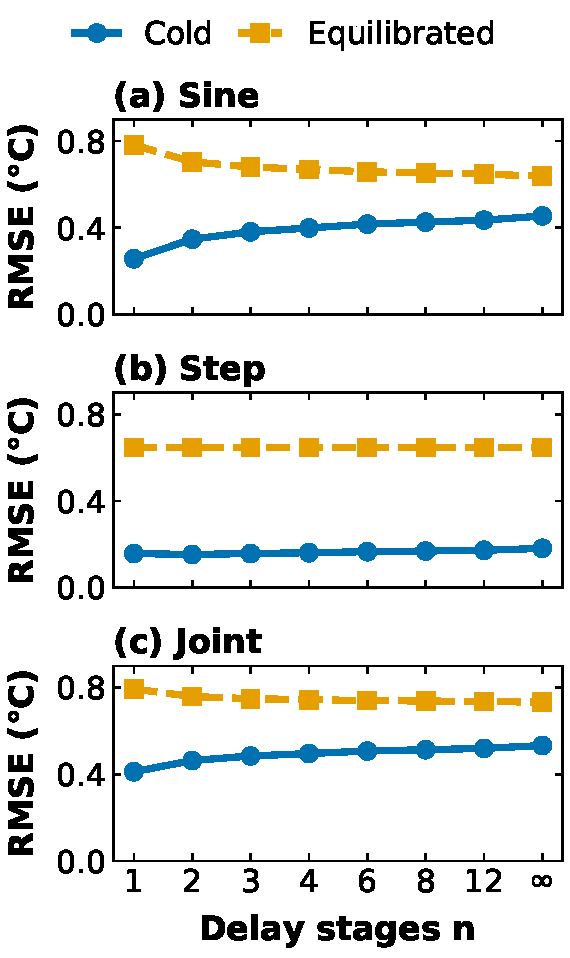
\includegraphics[width=.5\linewidth]{baseline_order.pdf}
 \caption{Initialization changes the fitted order ranking. Root mean squared
 temperature error (RMSE) for sine, step, and joint calibration is plotted for
 input--output parameter fits. Cold means $z_i(0)=0$; equilibrated means
 $z_i(0)=u(0)$. The infinity label denotes the separately fitted pure-delay model,
 with the corresponding input prehistory. Lines connect categorical orders as
 guides. Every error excludes the first temperature used to initialize the
 model. No uncertainty intervals are implied by the markers.}
 \label{fig:baseline-order}
\end{figure}

\subsection{Temperature traces and residuals}
The jointly calibrated cold models give closely spaced temperature predictions,
while their residual traces show differences near startup and the sine peaks
(Fig.~\ref{fig:baseline-trajectories}). Residual structure persists over many
successive observations. A visual match on the full temperature scale therefore
does not establish independent sensor noise or reliable uncertainty coverage.

\begin{figure}[p]
 \centering
 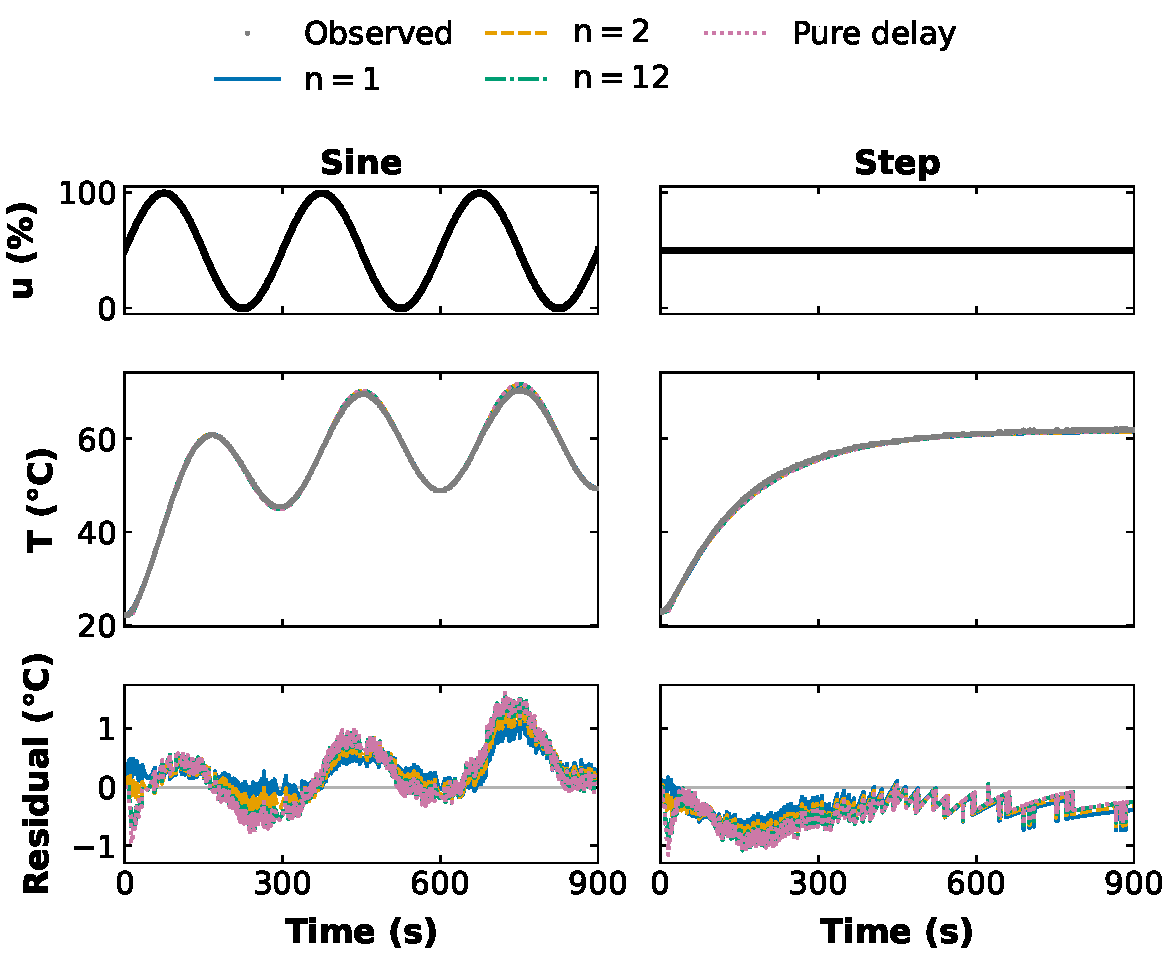
\includegraphics[width=\linewidth]{baseline_trajectories.pdf}
 \caption{The residual scale exposes differences hidden in the temperature
 overlays. Columns show the sine and step experiments; rows show heater input
 $u$, measured temperature $T$ with jointly fitted cold-start mean predictions,
 and residuals defined as prediction minus observation. All recorded calibration
 samples are plotted. The thermal initial condition and assumed ambient equal
 the first observation, and the delay prehistory is zero. The four curves use
 independent joint fits for their respective formulations. These are mean
 predictions; uncertainty bands are not shown.}
 \label{fig:baseline-trajectories}
\end{figure}

\subsection{Coordinate conditioning and physical ambiguity}
The independently fitted physical and input--output formulations reach sums of
squares that agree to numerical precision in the joint cold cases
(Table~\ref{tab:coordinate-metrics}). Reexpressing the same sensitivity matrix
changes its condition number. Moment coordinates do not improve this particular
metric at these fitted points. These differences concern the coordinate metric;
they do not distinguish observationally equivalent model explanations.
% Generated by render_tables.py; edit the producer, not this table.
\begin{table}[tbp]
\centering
\small
\begin{tabular}{lrrrr}
\toprule
Model & IO logs & Physical logs & Moment & $|\Delta S|$ \\
\midrule
$n=1$ & 23.1 & 19.38 & 27.76 & $6.3\times10^{-12}$ \\
$n=2$ & 21.04 & 17.56 & 24.82 & $1.5\times10^{-11}$ \\
$n=3$ & 20.61 & 17.19 & 24.15 & $1.3\times10^{-12}$ \\
$n=4$ & 20.44 & 17.04 & 23.86 & $4.3\times10^{-11}$ \\
$n=6$ & 20.29 & 16.9 & 23.6 & $2.1\times10^{-11}$ \\
$n=8$ & 20.23 & 16.84 & 23.48 & $3.2\times10^{-12}$ \\
$n=12$ & 20.16 & 16.78 & 23.36 & $3.4\times10^{-13}$ \\
Pure delay & 20 & 16.64 & 23.09 & $8.0\times10^{-11}$ \\
\bottomrule
\end{tabular}
\caption{Coordinate metrics for joint cold fits. The first three columns are sensitivity condition numbers at the same IO model point, transforming the information matrix without refitting. Moment coordinates are $(\log K,\log m,\ell)$ with $m=\tau+\theta$ and $\ell=\log[\theta/\tau]$. The last column compares independently fitted IO and physical sums of squares, in squared degrees Celsius. Conditioning changes do not imply additional information.}
\label{tab:coordinate-metrics}
\end{table}


The original model has a stronger ambiguity. For each calibration, the saved
structural calculation sampled 403 positive physical parameter combinations with
the same transfer function. Their largest prediction difference was below
$1.8\times10^{-12}\,{}^\circ\mathrm C$. Conductance $\Ua$ remained fixed while
$\Ub$, $\CpH$ and $\CpS$ varied. Appendix~\ref{sec:structural} gives the
analytic family and its positivity limits; sampled ranges are not confidence
intervals.

The analytic family also exposed an interpolation failure. All nine redundant
physical-parameter profiles excluded some known equivalent family members from
their interpolated 95\% grid sets. The sampled objective values along the flat
region were correct; coarse interpolation across its rising edge produced the
misleading endpoints. We therefore withhold those endpoints as physical
confidence claims. The merged profile catalog records this finding separately
from the successful likelihood arithmetic and nuisance-fit checks. A converged
pointwise optimizer and a plotted crossing do not validate the whole profile set.

\subsection{Conditional delay uncertainty}
Table~\ref{tab:delay-uncertainty} compares delay uncertainty for representative
joint cold formulations. Increasing the residual block length widens the
percentile intervals relative to independent Gaussian simulation. The one-stage
profile has two accepted pole-label modes; canonical bootstrap summaries refer
to only the representative with $\tau\geq\theta$. A finite full-coordinate
interval is withheld where the recorded experiment leaves delay unobservable.
The table compares assumptions rather than estimating a single unconditional
physical uncertainty.
% Generated by render_tables.py; edit the producer, not this table.
\begin{table}[tbp]
\centering
\small
\begin{tabular}{lcccc}
\toprule
Model & IID profile set & IID simulation & Circular block 60 & OU local SD \\
\midrule
$n=1$ & $[16.35,16.76]\cup[150.2,151.2]$ & $[16.44,16.69]$ & $[15.62,17.56]$ & 0.585 \\
$n=2$ & $[15.2,15.6]$ & $[15.3,15.51]$ & $[14.31,16.44]$ & 0.606 \\
$n=12$ & $[14.41,14.82]$ & $[14.52,14.72]$ & $[13.25,15.98]$ & 0.654 \\
Pure delay & $[14.26,14.67]$ & $[14.38,14.56]$ & $[13.34,15.68]$ & 0.317 \\
\bottomrule
\end{tabular}
\caption{Joint cold delay uncertainty in seconds. Profile sets use a profiled common IID variance and retain both one-stage pole modes. Percentile intervals use 400 Gaussian simulations at fixed $\sigma=0.25$ degrees Celsius or 400 circular residual-block refits, respectively. Bootstrap one-stage delays use the canonical pole representative. OU entries are local standard deviations with variance profiled and length included in the Hessian, not interval endpoints. These procedures make different assumptions and are not interchangeable coverage guarantees.}
\label{tab:delay-uncertainty}
\end{table}


\subsection{The working correlated-noise model remains inadequate}
The independent innovations audit reproduced every saved OU likelihood within
$2.6\times10^{-12}$. This validates likelihood arithmetic, not the residual
model. Filtered innovations retain strong negative lag-one correlation
(Table~\ref{tab:ou-diagnostics}). The fitted length therefore cannot be treated
as a measured thermal disturbance time scale. Mean prediction errors on the
held-out records also remain much larger than calibration errors. Allowing
serial covariance changes conditional uncertainty without establishing that
the thermal mean transfers between records.
% Generated by render_tables.py; edit the producer, not this table.
\begin{table}[tbp]
\centering
\small
\begin{tabular}{lrrrr}
\toprule
Model & Length (s) & $\hat\sigma$ (${}^\circ$C) & ACF1, sine & ACF1, step \\
\midrule
$n=1$ & 17.46 & 0.4088 & -0.5333 & -0.492 \\
$n=2$ & 22.14 & 0.459 & -0.5291 & -0.4935 \\
$n=12$ & 27.91 & 0.5151 & -0.5253 & -0.4877 \\
Pure delay & 29.33 & 0.5289 & -0.518 & -0.4811 \\
\bottomrule
\end{tabular}
\caption{Working OU fits to the two joint cold records. The scale is the maximum-likelihood stationary residual standard deviation. ACF1 is the centered sample lag-one correlation of filtered innovations. Strong remaining negative correlation challenges this one-component residual covariance; a high fitted likelihood does not validate it.}
\label{tab:ou-diagnostics}
\end{table}


The remaining empirical results will be inserted after the independent coverage,
ambient/history sensitivity, validation and prospective-design audits finish.
\FloatBarrier

\section{Discussion}
The transfer-function analysis places a limit on what a better input can achieve.
Under the single measured output and fixed initial conditions, excitation cannot
separate the original model's equivalent physical parameter combinations.
Estimating the three transfer coefficients or measuring an additional independent
quantity is a different scientific task from narrowing a four-parameter local
covariance. The existing data include a second sensor, but its usefulness for
breaking this equivalence requires a model that connects that sensor to the
states; the second trace alone does not establish that connection.

Initialization is part of the model specification. A delay that appears estimable
under cold delay states may become unobservable under equilibrated delay states
and constant input. Future laboratory records should include the heater history
before the fitting window and an independent ambient measurement. These records
would reduce dependence on assumptions made at the first sample.

The remaining discussion will assess the completed resampling, held-out
prediction, numerical sensitivity, and prospective-design results. Conditional
precision under a chosen residual model must be considered alongside error on
experiments excluded from calibration.

\section{Data, code, and research status}
The repository source is \url{https://github.com/dowlinglab/pyomo-doe}, on branch
\texttt{reformulation-exploration}, under
\texttt{skunk\_works/delay\_study}. Phase manifests identify immutable source
commits, data hashes, configuration, environment, seeds, and numerical outcomes.
The final draft will name a verified release commit after all computations and
artifact checks finish. The supplied raw data and inherited source were preserved.

An OpenAI Codex agent performed the notebook exports, implemented the numerical
analysis, ran the computations, searched and inspected literature, and drafted
this document. This disclosure describes scientific and software work as well
as writing assistance. The document has not received human scientific review.
No laboratory hardware experiment was performed for this study, and no target
journal or submission policy has been selected.

\bibliographystyle{plainnat}
\bibliography{bibliography}
\appendix
\section{Structural derivations}
\label{sec:structural}

\subsection{Delay-chain moments and pure-delay limit}
Let $r=n/\theta$ be the delay-state rate. The normalized chain kernel for
$t\geq0$ is
\[
 h_n(t)=\frac{r^n t^{n-1}e^{-rt}}{(n-1)!}.
\]
Its Laplace transform is $(1+s/r)^{-n}$. Differentiating that transform at zero
gives mean $n/r=\theta$ and variance $n/r^2=\theta^2/n$. Consequently, the
normalized complete thermal response has impulse-time mean $\tau+\theta$ and
variance $\tau^2+\theta^2/n$. These are properties of the model kernel;
they are not estimates of a measured residence-time distribution.
For fixed $s$ in the domain of convergence,
\[
 \log(1+\theta s/n)^{-n}=-n\log(1+\theta s/n)\longrightarrow-\theta s.
\]
This calculation supplies the pure-delay limit of Eq.~\eqref{eq:transfer}.

\subsection{An explicit physical-parameter equivalence class}
Define the two positive pole time constants $t_{\mathrm f}<t_{\mathrm s}$ by
$a=t_{\mathrm f}+t_{\mathrm s}$ and $b=t_{\mathrm f}t_{\mathrm s}$. For fixed
positive transfer coefficients $(K,a,b)$, choose a family coordinate
$r=\CpS/\Ub$ between these pole time constants. The physical parameters
\begin{equation}
 \Ua=\frac{c}{K},\qquad
 \CpH=\frac{b\Ua}{r},\qquad
 \CpS=\Ua\left(a-r-\frac{b}{r}\right),\qquad
 \Ub=\frac{\CpS}{r}
 \label{eq:equivalent}
\end{equation}
produce exactly the same transfer function for every
$r\in(t_{\mathrm f},t_{\mathrm s})$. Positivity follows from
$a-r-b/r=-(r-t_{\mathrm f})(r-t_{\mathrm s})/r>0$. Substitution into
Eq.~\eqref{eq:original-transfer} recovers $K$, $a$, and $b$ exactly.
The conductance $\Ua$ is identifiable through $K$; the other three parameters
vary along this equivalence class. No input waveform can distinguish members
of this class through this output under the stated initial conditions.

Positivity constrains this continuum to finite ranges in some coordinates.
For example, its heat capacities obey
\[
 \Ua t_{\mathrm f}<\CpH<\Ua t_{\mathrm s},\qquad
 0<\CpS\leq\Ua\left(a-2\sqrt b\right).
\]
The second upper bound occurs at $r=\sqrt b$.
Thus bounded physical ranges or bounded exploration grids do not establish
structural identifiability. Structural uniqueness must be checked separately
from the numerical width of a confidence set.

\subsection{Constant input with equilibrated delay states}
If $u(t)=u_0$ and $z_i(0)=u_0$, every delay-state derivative in
Eq.~\eqref{eq:chain} vanishes. The predicted temperature then depends on
$K$ and $\tau$ alone, and its derivative with respect to $\theta$ is zero at
every observation time. A constant prehistory gives the same conclusion for
Eq.~\eqref{eq:puredelay}. This experiment cannot estimate the delay even when
the thermal transient is well measured. Cold delay states under the same
post-start input retain a transient that depends on $\theta$.

\subsection{Coordinate changes and information}
For positive parameters, write $\bm\eta=(\log K,\log\tau,\log\theta)^\top$
and $\bm\xi=(\log\Ua,\log\Cp,\log\theta)^\top$. The Jacobian of the map
from $\bm\eta$ to $\bm\xi$ is the constant matrix
\[
 M=\begin{pmatrix}-1&0&0\\-1&1&0\\0&0&1\end{pmatrix},\qquad M^{-1}=M.
\]
For a nonsingular covariance $C_{\eta}$, the transformed local covariance is
$C_{\xi}=M C_{\eta}M^\top$. Sensitivity rank and prediction-space uncertainty
are invariant under this invertible transformation. Numerical eigenvalues,
eigenvectors, and condition numbers generally change with the coordinate metric.
The matrix satisfies $|\det M|=1$, so log-coordinate information determinants
at the same model point are equal in this particular transformation.

\section{Literature coverage and claim audit}
The review used the configured lab literature skill and project-oriented searches
of the local library, followed by primary-source web discovery. It is a focused
review, without an exhaustive database search or a formal systematic-review
protocol. Search passages that only list another work in their references were
excluded as support for that work's claims.

The source record \texttt{literature/source\_review.json} retains paper identities,
source events where available, physical-page locators, and claim limitations.
The record \texttt{literature/acquired\_sources.json} identifies downloaded PDFs
by their hashes. Full paper text and PDFs remain outside this repository.

The Raue et al. source has library paper identifier
\texttt{6925c25f}\ldots\texttt{ae8160}; the inspected profile construction is
on physical PDF page 4, printed page 1926, Eq.~(10). The Hjalmarsson journal
source was checked at physical pages 8--9, printed pages 282--283, for confidence
regions, identifiable combinations, and the assumptions behind prediction-error
information. Those two pages were also inspected as rendered images because
the extraction engines disagree on equation symbols. The Hurtado--Kirosingh
journal source was checked at physical pages 11--12, printed pages 1841--1842,
for the chain equations and their integral-equation equivalence, with rendered
page inspection of the mathematical passages.

The downloaded adaptive-input-design preprint changes title and author order
relative to its published journal record. Its publication version remains under
review and it is not yet cited for a theorem. A continuous-time-identification
book search returned relevant pages, but chapter authorship remains unverified;
that content is not yet attributed to the volume editors. These holds will remain
visible until the corresponding sources have been checked.

\end{document}
